\chapter{Results}

% TODO: talk about AlexNet (78 AlexNet-like models, 5.10dB)
\section{LeNet-Like CNNs}

  I trained and beamformed over 1000 LeNet-like models generated with our constraint-satisfaction random search. The best performing LeNet has an average CNR of 5.46dB with a standard deviation of 0.45dB. The architecture and hyperparameters of the best-performing model is as follows:

\begin{table}[]
\vspace*{5mm}
\centering
\renewcommand\arraystretch{0.9}
\begin{tabular}{@{}ll@{}}
% \toprule
Hyperparameter & Value \\ \midrule
Architecture Type & LeNet-like \\
Input Formulation & 1x130x1 \\
Using Max Pooling & True \\
Using Batch Normalization & True \\
Adding Gaussian Noise & True \\
Conv1 Kernel Size & 17 \\
Conv1 Number of Kernels & 45 \\
Conv1 Stride & 1 \\
Conv1 Dropout & 0 \\
Pool1 Kernel Size & 2 \\
Pool1 Stride & 2 \\
Conv2 Kernel Size & 12 \\
Conv2 Number of Kernels & 35 \\
Conv2 Stride & 1 \\
Conv2 Dropout & 0.5149 \\
Pool2 Kernel Size & 2 \\
Pool2 Stride & 2 \\
Fully-Connected (FC) Layers & 2 \\
FC Layers Width & 109 \\
Loss Function & Smooth Mean Absolute Error \\
Optimizer & Adam \\
Learning Rate & 1.803e-4 \\ \bottomrule
\end{tabular}
\vspace{0.5mm}
\caption{Architecture and hyperparameters for the best LeNet model}
% \label{tab:my-table}
% \vspace{-10mm}
\end{table}


  I found that LeNet-like CNNs featuring two convolutional layers and two or three fully-connected layers were effective in suppressing off-axis noise. I also found that adding Gaussian noise in training was useful. Furthermore, for LeNets, it was better to concatenate the I and Q components as a single-channel 1D array or stack them as a two-channel 1D array than to stack them as a one-channel 2D array. Furthermore, almost all top-performing models used Adam instead of SGD as their optimizers. In terms of loss functions, L1 was ineffective compared with MSE and Smooth L1.

  For phantom targets, the CNR was 5.46$\pm$0.45 dB, 5.57$\pm$0.20 dB, and 4.24$\pm$0.38 dB for the best LeNet, the best MLP, and DAS, respectively. A qualitative assessment of the speckle pattern at the top of the phantom images suggest that LeNets introduce less intereference farther away from the focus, suggesting a potential benefit of having a larger depth of field.

  \begin{figure}[htbp]
    \centerline{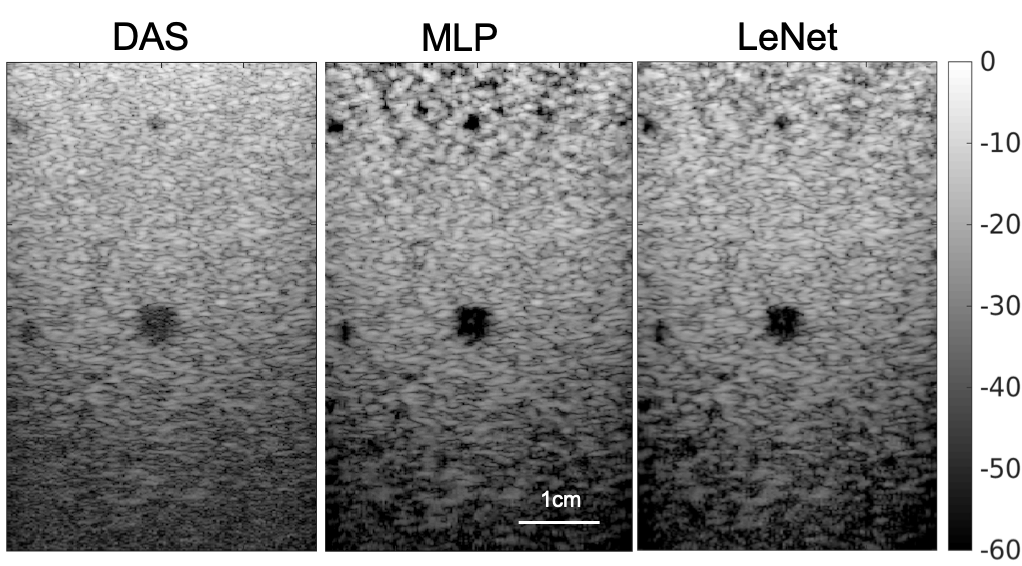
\includegraphics[width=85mm,scale=0.5]{phantom_das_mlp_lenet.png}}
    \caption{For a phantom target, DAS has a CNR of 4.40, MLP 5.54, LeNet 5.29}
    \label{fig}
  \end{figure}


  In addition, like the best MLP, the best LeNet is able to translate its phantom CNR improvements to \textit{in vivo} scans.
  \begin{figure}[htbp]
    \centerline{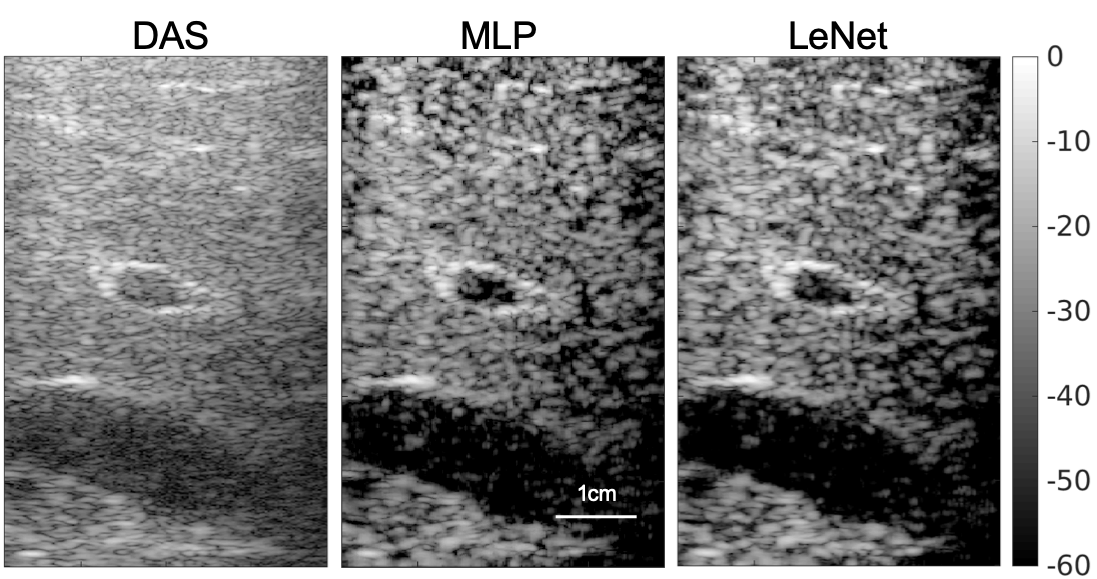
\includegraphics[width=85mm,scale=0.5]{in_vivo_das_mlp_lenet.png}}
    \caption{For an in vivo target, DAS has a CNR of -14.98, MLP -0.80, LeNet -2.84}
    \label{fig}
  \end{figure}


  A t-test was used to compare the phantom CNR value for all scan targets between the best LeNet and the best MLP. The difference was not statistically significant, with a p-value of 0.45. This finding suggests that LeNets produce equivalent results to MLPs. A plot of CNR values as a function of the total number of model weights also shows that LeNets approximate the performance of MLPs with two magnitude fewer weights. This could potentially mean that LeNets are easier to train and faster to deploy compared with MLPs.

  \begin{figure}
    \centerline{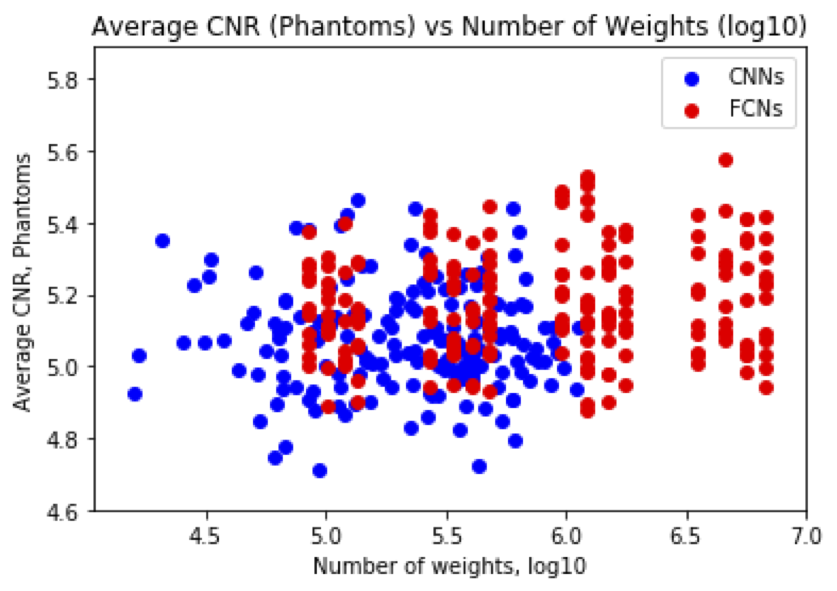
\includegraphics[width=85mm,scale=0.5]{avg_cnr_vs_num_weights.png}}
    \caption{The best LeNets tend to have fewer weights than the best MLPs}
    \label{fig}
  \end{figure}


\section{FCNs}
\subsection{Overview}
  I also trained and beamformed 450 FCNs with the best-performing model having an average CNR of 4.93dB and a standard deviation of 0.20dB. The architecture and hyperparameters of the best-performing model is as follows:

  \begin{table}[]
  \vspace*{5mm}
  \centering
  \renewcommand\arraystretch{0.9}
  \begin{tabular}{@{}ll@{}}
  % \toprule
  Hyperparameter & Value \\ \midrule
  Architecture Type & FCN-4 \\
  Input Formulation & 1x65x2 \\
  Using Batch Normalization & False \\
  Adding Gaussian Noise & True \\

  Conv1 Kernel Size & 13 \\
  Conv1 Number of Kernels & 59 \\
  Conv1 Padding & 3 \\
  Conv1 Stride & 2 \\

  Conv2 Kernel Size & 4 \\
  Conv2 Number of Kernels & 36 \\
  Conv2 Padding & 2 \\
  Conv2 Stride & 2 \\

  Conv3 Kernel Size & 6 \\
  Conv3 Number of Kernels & 19 \\
  Conv3 Padding & 3 \\
  Conv3 Stride & 1 \\

  Conv4 Kernel Size & 6 \\
  Conv4 Number of Kernels & 2 \\
  Conv4 Padding & 2 \\
  Conv4 Stride & 1 \\


  Loss Function & Smooth Mean Absolute Error \\
  Optimizer & Adam \\
  Learning Rate & 1.0e-5 \\ \bottomrule
  \end{tabular}
  \vspace{0.5mm}
  \caption{Architecture and hyperparameters for the best FCN model}
  % \label{tab:my-table}
  % \vspace{-10mm}
  \end{table}

  For phantom targets, the CNR was 4.93$\pm$0.20 dB for the best FCN model, offering a modest improvement over DAS (4.24$\pm$0.38 dB). Visually, the FCN is unable to improve the contrast of the structures at the top of the phantom.

  \begin{figure}[htbp]
    \centerline{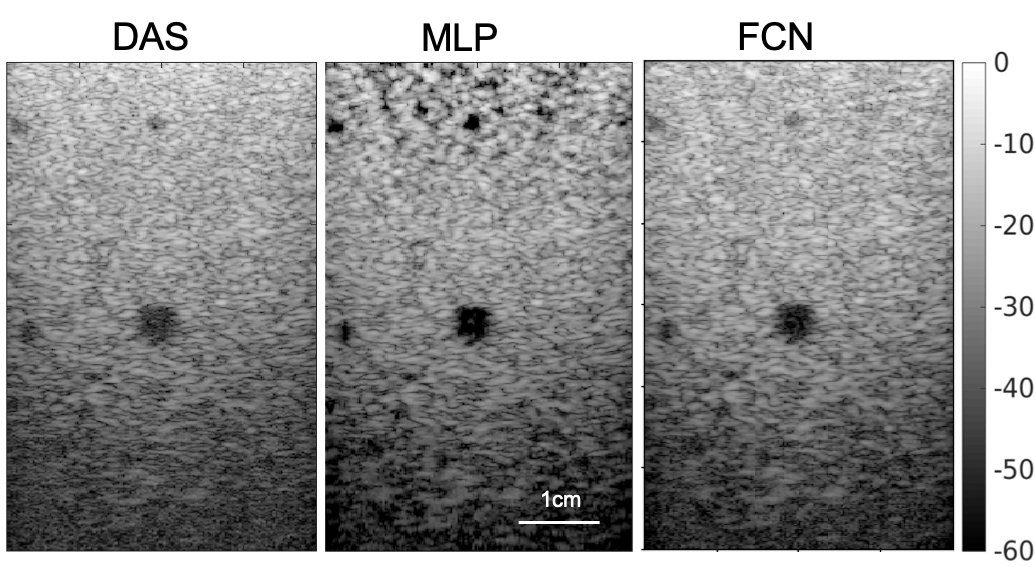
\includegraphics[width=85mm,scale=0.5]{phantom_das_mlp_fcn.png}}
    \caption{For a phantom target, DAS has a CNR of 4.39, MLP 5.54, FCN 4.87}
    \label{fig}
  \end{figure}

  For \textit{in vivo} targets, the FCN beamformed image has a modest contrast improvement over the DAS image. A qualitative assessment indicates that the smaller vascular features are not as clear in the FCN image as in the MLP beamformed image.


  \begin{figure}[htbp]
    \centerline{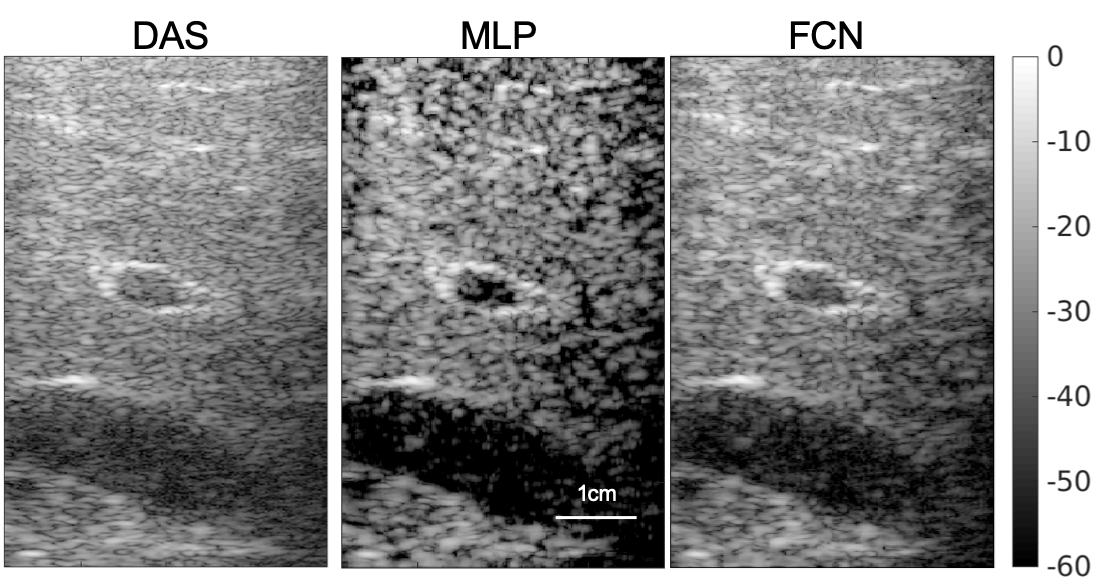
\includegraphics[width=85mm,scale=0.5]{in_vivo_das_mlp_fcn.png}}
    \caption{For an in vivo target, DAS has a CNR of -14.98, MLP -0.80, FCN -5.92}
    \label{fig}
  \end{figure}

  The full range of models performance for FCNs with outliers, as a function of the log number of weights, is shown in Figure \ref{fig:cnr_vs_num_weights_fcns_mlps}. The same distribution without outliers is shown in Figure \ref{fig:cnr_vs_num_weights_fcns_mlps_no_outliers}.

  \begin{figure}[htbp]
    \centerline{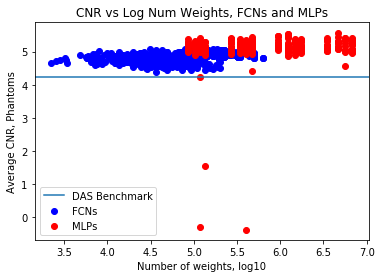
\includegraphics[width=85mm,scale=0.5]{cnr_vs_num_weights_fcns_mlps.png}}
    \caption{Phantom average CNR as a function of the log number of weights (with outliers), FCNs and MLPs}
    \label{fig:cnr_vs_num_weights_fcns_mlps}
  \end{figure}

  \begin{figure}[htbp]
    \centerline{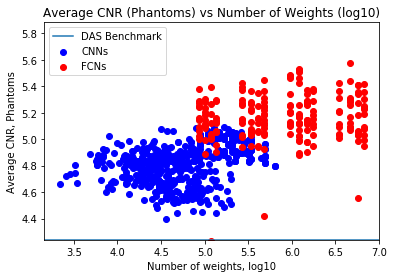
\includegraphics[width=85mm,scale=0.5]{cnr_vs_num_weights_fcns_mlps_no_outliers.png}}
    \caption{Phantom average CNR as a function of the log number of weights (without outliers), FCNs and MLPs}
    \label{fig:cnr_vs_num_weights_fcns_mlps_no_outliers}
  \end{figure}

% TODO: show all the models.
% TODO: Show another architecture: FCN-N
% \subsection{Phantom CNR vs. Kernel Size}
% Waiting for more results.
% % We investigated the relationship between the kernel size and the average CNR value.
% %
% % \begin{figure}
% %   \centerline{\includegraphics[width=85mm,scale=0.5]{cnr_vs_num_conv_layers.png}}
% %   \caption{The best CNNs tend to have fewer weights than the best FCNs}
% %   \label{fig}
% % \end{figure}
%
% \subsection{Phantom CNR vs. Number of Convolutional Layers}
% Waiting for more results.
%
% \subsection{FCNs with Same Number of Weights}
% Waiting for more results.
%
% \section{Bottlenecked MLPs}
% Waiting for more results.

% \section{Loss Curves}
% Even though we do not rely on loss for model selection, it is helpful to visualize the learning process.
%
% We can see that the loss curve is rather short. Perhaps they never learned?
%
%
